\documentclass{article}
\usepackage[utf8]{inputenc}
\usepackage[T1]{fontenc}
\usepackage{hyperref}
\usepackage{todonotes}
\usepackage{gensymb} % superscript
\usepackage{textcomp} % superscript
\usepackage{amsmath} % symboles des degrés

% --------------------  NOMBRES ET UNITÉS ---------------------------
\usepackage{siunitx}
\iffalse % explication des fonctions courantes
The package provides the user macros:
• \ang[hoptionsi]{hanglei}
• \num[hoptionsi]{hnumberi}
• \si[hoptionsi]{huniti}
• \SI[hoptionsi]{hnumberi}[hpre-uniti]{huniti}
• \numlist[hoptionsi]{hnumbersi}
• \numrange[hoptionsi]{hnumbersi}{hnumber2i}
• \SIlist[hoptionsi]{hnumbersi}{huniti}
• \SIrange[hoptionsi]{hnumber1i}{hnumber2i}{huniti}
• \sisetup{hoptionsi}
• \tablenum[hoptionsi]{hnumberi}
plus the S and s column types for decimal alignments and units in tabular environments.
12 345.678 90        \num{12345,67890}
1 ± 2i               \num{1+-2i}
0.3 × 1045           \num{.3e45}
1.654 × 2.34 × 3.430 \num{1.654 x 2.34 x 3.430}

\si{kg.m.s^{-1}}
kg m s−1
Simple lists and ranges of numbers can be handled.
\numlist{10;20;30} \\
\SIlist{0.13;0.67;0.80}{\milli\metre} \\
\numrange{10}{20} \\
\SIrange{0.13}{0.67}{\milli\metre}
10, 20 and 30
0.13 mm, 0.67 mm and 0.80 mm
10 to 20
0.13 mm to 0.67 mm

\ohm\metre
\celsius

\fi
% --------------------------------------------------------------

\usepackage{hyperref}

\usepackage{natbib}       % Pour la bibliographie
\usepackage[french]{babel}
\usepackage{graphicx}     % Pour les figures
\usepackage[toc]{appendix}% Pour les annexes
\usepackage{titlesec}     % Pour modifier les titres
\usepackage{fancyhdr}     % Pour les haut et bas de pages (numéros)
\usepackage{lipsum}       % Rajoute du texte temporaire
\usepackage{parskip}      % Modifie l'apparence des paragraphes
\usepackage{setspace}     % Pour interligne et demi
\usepackage{listings}     % Pour afficher du code sans formattage

\selectlanguage{french}

% ------------------------- COMMANDES -------------------------------

\newcommand\var[2]{\newcommand{#1}{\ensuremath{#2}}}
% C'est pratique de définir des variables au début pour éviter de
% réécrire des formules et cela facilite modifier l'affichage.

\makeatletter
\newcommand{\makecustomtitle}{
  \newpage
  \null
  \begin{center}
  \let \footnote \thanks
    {\LARGE \textbf{\@title} \par}
    \vskip 1em
    {\large \@date \par}
    \rule{1.5in}{0.4pt}
  \end{center}
  \par
}
\makeatother


\title{Auto}
\author{pascal.rainville }
\date{January 2019}

\begin{document}

\maketitle

\section{Batterie}

Le voltage ne devrait jamais baisser plus bas que 80\% de charge. Donc, la batterie ne devrait jamais être plus basse que 12.4V. À vérifier 1 fois par semaine, l'hiver les grosses semaines de froid. Plus la charge baisse, plus il est possible que la batterie gel. Une batterie qui gèle devrait pratiquement scrap. En bas de 40\% de charge, elle peut geler assez facilement.

Le starter de 1.6kW à 12V requiert 133A. La batterie est de 

Je n'arrive pas à trouver le nombre d'A*h. J'aurais aimé savoir le nombre de fois que je peux démarrer ma voiture.

CA: cranking amps: 550A (30s à 0 celcius)
CCA: cold cranking amps: 675A (30s à -18 celcius)

Open Cell Voltage
The difference in electrode potential at zero current density is called the open cell voltage at a given state-of-charge, as shown by the previous figure.

The open cell voltage for a battery as a function of temperature at a given state-of-charge is calculated by the following expression:

(1)

where  is the cell voltage,  is the entropy change of the battery reaction,  is the number of electrons transferred, and  is the Faraday constant. This means that for a battery with a net discharge reaction with a positive entropy change (), the cell voltage increases with temperature. For a battery with a negative entropy change, the cell voltage decreases as temperature increases.

Most lithium-ion batteries used in modern electric vehicles have a slightly negative or a very small entropy change, which means that the open cell voltage increases slightly as temperature decreases. This alone would actually improve performance at lower temperatures. However, the change in open cell voltage as a function of temperature is relatively small compared to other parameters, around 0-0.4 mV/K — that is less than 30 mV over a range of very cold temperatures (-35°C, -31°F) to room temperature. We can therefore rule out the net discharge reaction thermodynamics as a reason for poor performance at low temperatures.

https://www.comsol.com/blogs/why-car-batteries-perform-poorly-in-cold-weather/

Bref: La température n'affecte pratiquement pas le voltage de la batterie.

A standard small car battery is about 45 amp*hours.

\begin{figure}[h]
    \centering
    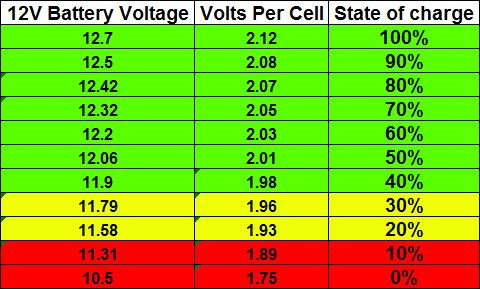
\includegraphics[scale=0.5]{figureVoltageBatterie.jpg}
    \caption{Charge de la batterie selon le voltage}
    \label{fig:my_label}
\end{figure}
Source: https://i.pinimg.com/originals/be/e3/3e/bee33e3900f485e036ab48387b4b2e54.jpg

\section{Alternateur}

Most cars, while the engine is running, have a charging system that will generally
produce a voltage between 13.5 and 14.4 volts.  to overcome the internal resistance of the
battery.

The actual output voltage produced by the alternator
will typically be about 1-1/2 to 2 volts higher than battery voltage. At idle, most charging
systems will produce 13.8 to 14.3 volts with no lights or accessories on. 

J'ai lu quelque part que si l'alternateur output 15V, ça peut tuer la batterie.

Source: imental study on the effect of alternator
speed to the car charging system
Rozdman K. Mazlan1,*, Reduan M. Dan1,2, Mohd Z. Zakaria1,2, Abdul H. A. Hamid1
1
Faculty of Mechanical Engineering, Universiti Teknikal Malaysia Melaka, Hang Tuah Jaya, 76100
Durian Tunggal, Melaka, Malaysia.
2
Centre for Advanced Research on Energy, Universiti Teknikal Malaysia Melaka, Hang Tuah Jaya,
76100 Durian Tunggal, Melaka, Malaysia.
Abstract. In this paper, we present our work, which is doing an energy 
https://www.matec-conferences.org/articles/matecconf/pdf/2017/04/matecconf_aigev2017_01076.pdf

\section{Écho 2003}

\subsection{changement d'huile}

Dernier:
Prochain:

\subsection{Changer le starter}

Ratchet 14mm avec moyenne ralonge 3/8 pour la vis du haut.
Ratchet 12mm et clé 12 mm pour celle du bas.
Ratcher 1/2 pour vis du connecteur électrique.
Déplugger l'autre fil.

Le starter est de 1.6 kW. À 12V, c'est 133.33 A. Ça veut dire que j'aurais pu acheter un car booster de 200A et partir mon auto sans même avoir une batterie... Peut-être ça dépend de la durée du 200A...

\subsection{Freins à tambour}

\subsection{Huiles}
Huile à moteur:
Fluide à frein: SAE J1703 or FMVSS No.116 DOT 3

\subsection{Jacker le char}

Il y a 4 points pour lever avec le jack pantograph (celui qui vient avec l'auto j'imagine). Sinon il y a un place au centre en avant et une place au centre en arrière pour lever l'avant et l'arrière en même temps. À voir. Il y a une image dans le owners manual.

\end{document}
